\chapter{General Lab Procedures}
The following is basic procedures and guidelines that students should follow when performing certain actions in the lab.  These guidelines are meant as a starting point for students when working on their construction projects in the lab.  These are not meant to be a comprehensive guide, but should help students in getting started.  If you still have questions or concerns on a certain procedure, please visit with a lab monitor, lab technician or the M:2:I Program Coordinator.

\section{Sanding Procedures}
Sanding is a method in which we remove material from the object we are working with.  This is often needed in order to smooth the object, refine the shape, or even polish an object.

\begin{framed}
\begin{wrapfigure}{L}{0.14\linewidth}

\includegraphics[width=\linewidth]{images/important_icon.png}
\end{wrapfigure}
\ \\
Sanding will generate fine particulate matter that can be irritating to the skin eyes, or lungs.  Students sanding must wear eye protection and in most cases must wear a face mask to prevent this irritation.  Use of a downdraft table will also help minimize irritation.
\end{framed}
Sandpaper comes in many different grits. The higher the number of the grit, the finer the sandpaper. This lab has sandpaper that ranges from 60 grit to 1500 grit. When sanding, start at a lower grit number and step up one grit increment at a time until the desired surface finish is reached. 

All sandpaper is locked up in the tool crib and must be checked out by a lab monitor. It is up to you to understand what grit requirement you need and how to properly use sandpaper. The rest of this section will go over how to use sandpaper and grit numbers properly for different materials. If any questions remain, consult a lab monitor and they will recommend the correct grit and sanding procedure.

\subsection{Downdraft Table}
Groups that need to sand \emph{must} do so on the provided downdraft table. The M:2:I lab has one downdraft tables that groups may use for sanding or any activity that may produce small particulate.  To use the downdraft table, please follow the steps below.

\begin{enumerate}
\item Turn the power switch into the \textbf{ON} position. This is the left hand switch that is labeled \textit{Power}
\item Select the desired speed on the right hand switch labeled \textit{Speed}. The up position is \textbf{HIGH} and the down position is \textbf{LOW}
\item Sand on the top surface of the machine
\item If dust is not being pulled into the machine
\begin{enumerate}
\item Change the speed setting to \textbf{HIGH} if it is not already
\item If the speed is on \textbf{HIGH} and the dust is still not being collected, consult a lab monitor, the filter may be in need of replacement
\end{enumerate}
\item When finished sanding, sweep any remaining dust into the collection system prior to turning the power off
\item Turn the power switch into the \textbf{OFF} position
\item Clean up the immediate area
\end{enumerate}

If you have any questions about the downdraft tables or the tables are not working properly, see a lab monitor.  It also the responsibility of the user to clean up any material did not get pulled into the downdraft table.  Always clean up both on top of and around the downdraft table when finished.

\subsection{Wood}
Wood sanding procedure depends a lot on the type of wood being sanded. The most common used in the lab is oak, a hardwood, and balsa, a softwood.  The desired finish that the user wants also plays an important role, so it is important to know both the wood you are working with and what you want in the end.  Always make a plan on what you want to accomplish.  The following is some guidelines in making this plan.
\begin{enumerate}
\item Determine the type of wood that is going to be sanded
	\begin{enumerate}
	\item Hardwoods will require a lower starting grit whereas softwoods can use a finer grit to start with
	\item For most applications, starting with a 60 or 80 grit sandpaper is sufficient, for softwoods, using 100 grit to start with will also work.
	\end{enumerate}
\item Determine the type of finish required
	\begin{enumerate}
	\item If the wood needs to have a very fine finish, it will require more sanding and will require more steps between start and finish
	\item If the wood's finish is not entirely critical, only a few steps will be needed to achieve an acceptable finish
	\end{enumerate}
\item Start with an acceptable sanding grit and sand with the wood grain until the surface has a uniform look and feel
	\begin{enumerate}
	\item Use a piece of sandpaper until there is very little grit left on it or until the amount of material the sandpaper is removing is minimal, replace when the sandpaper is at this state
	\item When sanding with sandpaper, do not fold the sandpaper as this ruins the grit on one side, effectively wasting sandpaper
	\end{enumerate}
\item Depending on your requirements, step up to the next grit of sandpaper
	\begin{enumerate}
	\item Usually, if the starting grit was a 60, the next step up would be an 80. If its 80, the next step would be 100 and etc
	\end{enumerate}
\item Sand with each grit until the surface has achieved a smooth, uniform appearance before moving on to the next grit
\item Stop sanding when the surface has achieved an acceptable finish
\end{enumerate}

\subsection{Foam}
Sanding foam is quite different than sanding wood. Foam is much softer and does not require quite as low a starting grit and requires fewer steps from start to finish.  As with wood though, plan your actions to minimize wasting time and materials.
\begin{enumerate}
\item Generally 100 or 150 grit sandpaper is sufficient to sand foam and to get it to its desired shape.
\item Sand the foam until it reaches its desired shape
	\begin{enumerate}
	\item Since foam is much softer than wood, sanding will take much less time and require less effort
	\item Rarely will it be necessary to sand foam with sandpaper of a higher grit than 150
	\end{enumerate}
\item For most applications, one grit should be sufficient, however for finer finishes it may be necessary to use a second grit
\end{enumerate}

\subsection{Metal}
Unlike sanding both foam and wood, sanding metal removes very little material and is meant solely to provide surface finish. Sanding metal will require a great deal of time and effort. Metal also requires lower starting grits and more steps between start and finish than both wood and foam.
\begin{enumerate}
\item Determine current surface quality
	\begin{enumerate}
	\item It may be necessary to prepare the surface with a wire brush or grinder in order to remove surface obstructions and rust
	\end{enumerate}
\item Determine the finish that is necessary
	\begin{enumerate}
	\item Smooth surfaces require much less work than mirror like surfaces
	\end{enumerate}
\item Start with a relatively rough sandpaper to begin with. Generally a 60 grit should be sufficient
\item Sand until the surface has a uniform appearance
\item Step up to the next available grit and continue to sand until the surface scratches have been removed
\item Continue to sand and step up from grit to grit until the desired surface finish is reached
\begin{enumerate}
	\item To achieve a shiny, mirror-like surface, grits up to and in excess of 600 grit will likely be needed
\end{enumerate}
\end{enumerate}
\begin{framed}
\begin{wrapfigure}{L}{0.15\linewidth}

\includegraphics[width=\linewidth]{images/info_icon.png}
\end{wrapfigure}
\ \\
Iron metals have a thin layer called scale built up on the exterior of the metal. If a very shiny surface is desired, this layer will have to be completely removed. To do this a protective coating must be applied or the metal will oxidize.  This will undo all the work that was done to the part.  
\end{framed}
If you have further questions about working with metals, see the Program Coordinator or a lab monitor.

\section{Chemical Procedures}
Certain chemicals may also be used in the lab to achieve your final result in your construction.  These chemicals are often adhesives, etching, or painting.  As with any chemical, care must be taken when using these chemicals and all safety procedures must be observed.

\subsection{Adhesives}
Adhesives are frequently used in the Make to Innovate lab. When using adhesives, read all applicable labels and understand how the adhesive works. Seek a lab monitor's assistance if you are unsure as to how to use the adhesive correctly. Prior to using any adhesive, put down disposable paper or cardboard on the work surface being used to prevent spills or drips. Any spills or drips will be the responsibility of the student to clean up. Any subsequent damage resulting from improper use of adhesives will result in disciplinary actions.
\begin{framed}
\begin{wrapfigure}{L}{0.16\linewidth}
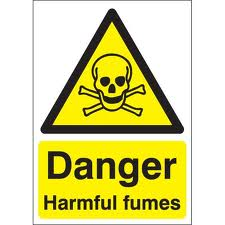
\includegraphics[width=\linewidth]{images/fumes_hazard.jpg}
\end{wrapfigure}
\ \\
Almost all adhesives produce fumes that can be harmful or toxic to humans.  Adhesives must be used in a well ventilated area.  Many of these fumes are also flammable, therefore they must be used away from any kind of ignition source.
\end{framed}
\subsection{Painting}
The Make to Innovate lab has brush-on paint available for use by groups. Painting can be done in the lab on the workbenches with lab monitor approval. All painting must be done on cardboard or paper to prevent spills. All spills must be cleaned up by groups immediately. Projects must have travelers affixed to their project if the project is to be left out to dry. 

Spray paints are prohibited in the lab. Make to Innovate will not supply spray paints, and groups are not allowed to bring in their own spray paints.  If spray paining must be used, permission must be obtained from the M:2:I Program Coordinator.  Spray painting is only permitted outside of Howe hall with proper PPE used and proper protection of the grass or concrete surface.  
\begin{framed}
\begin{wrapfigure}{L}{0.16\linewidth}
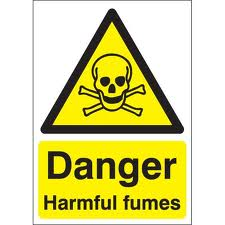
\includegraphics[width=\linewidth]{images/fumes_hazard.jpg}
\end{wrapfigure}
\ \\
Almost all paints produce fumes that can be harmful or toxic to humans.  Paints must be used in a well ventilated area.  Many of these fumes are also flammable, therefore they must be used away from any kind of ignition source.
\end{framed}